\chapter{Theoretical frame}
\label{chap:ch1}

\section{HTTP}

\par HTTP (Hypertext Transfer Protocol) is an application layer protocol in the Internet protocol suite model (TCP/IP) for data exchange in a client-server interaction. Messages sent by the client are called requests and the answers they receive from the server are called responses. 

\begin{figure}[!ht]
    \centering
    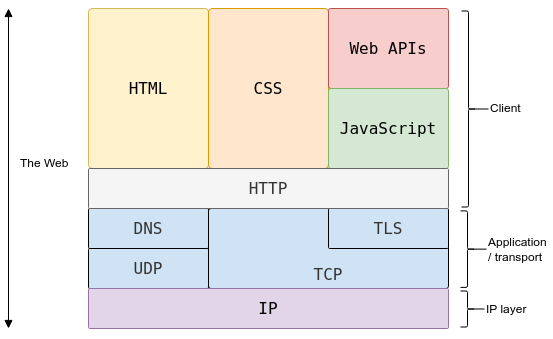
\includegraphics[width=1\linewidth]{web-layering.png}
    \caption{The web from the client layer to the IP layer \cite{httpOverviewLayers} }
    \label{fig:enter-label}
\end{figure}

\section{REST}

\par REST (Representational State Transfer) is an architectural style for designing network-based applications, particularly web services and is most used by HTTP client-server applications. It was introduced by Roy Thomas Fielding in 2000 for his doctoral dissertation. \cite{restPaper}

\par The architecture is defined by the following constraints:

\begin{enumerate}
    \item Client-Server - the separation of client and server gives each of them more portability, flexibility and thus leverages the scaling of the applications. This also increases cohesion within each side and decreases coupling between them. Having each of them deal with their own concerns also follows the Single Responsibility Principle of SOLID. 
    \item Stateless - every client request contains enough information in order for the server to understand and process the request. Only the client stores session state. This simplifies the work of the server.
    \item Cache - requiring the implicit or explicit labelling of the response as cacheable or non-cacheable in order to improve of network efficiency
    \item Uniform Interface - means having an uniform interface between the client and the server and implies:
    \begin{itemize}
    \item identification of resources - URI are used to identify resources and those resource are different from the representation sent to the client since a single resource can have multiple representation
    \item manipulation of resources through representations - if a client holds a representation of some resource, it has enough information to modify or delete it, provided they have access
    \item self-descriptive messages - messages contain enough information to describe how they should be processed (example: specifying the media type)
    \item hypermedia as the engine of application state - other resources can be accessed by the hyperlinks provided by the server
    \end{itemize}
    \item Layered System - a client can only see the immediate layer they are interacting with. Whether that layer is the final service or an intermediary is known
    \item Code-On-Demand (optional) - extending client functionality by downloading and executing code as applets/scripts.
\end{enumerate}

\par Throughout the application, the JSON representation (visible in Figure \ref{fig:json-example}) will be used for client-server interactions.

\begin{figure}[!ht]
    \centering
    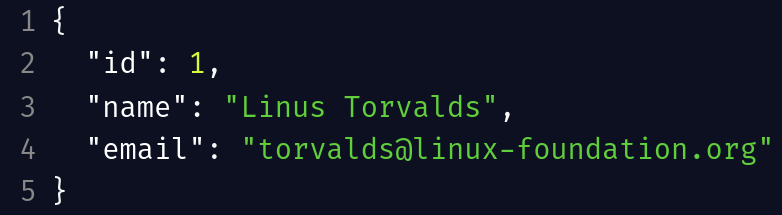
\includegraphics[width=1\linewidth]{json-example.png}
    \caption{Example of JSON serialized data}
    \label{fig:json-example}
\end{figure}

\section{Middleware}

\par Middleware is code that runs between the incoming HTTP request and the outgoing HTTP response. It is used to process requests and responses, handle specific tasks and make modifications before the request finally reaches the handler outside the middleware pipeline  or the response is sent back to the client.

\par Use cases for middleware

\begin{itemize}
    \item request processing - inspection, modification or rejection of incoming HTTP request before they reach their final handler. Examples: JSON parsing, handling file uploads, checking specific headers.
    \item authentication and authorization - examples: verify credentials or enforce role-based access controls
    \item logging and monitoring - examples: logging requests/response and error tracking
    \item error handling - it can catch and handle errors that occur during request processing and allows customization of the error messages and the http status codes returned to the client
    \item rate limiting and throttling - example: limit the number of requests/time in order to prevent abuse
    \item data transformation - modifying requests and responses by converting formats, adding default values or transforming the data before they reaches the final handler or are returned to the client 
\end{itemize}

\section{The Software Development Life-cycle}

\par The Software Development Life-cycle (SDLC) is the process that development teams go through in order to create a software product, from gathering the client's requirements till the end of their collaboration for that software's purpose.

The steps involved in SDLC may differ from team to team but a common denominator can be found among the following:

\begin{enumerate}
    \item Planning - involves analyzing the cost-benefit, scheduling, resource estimation and resource allocation. Requirements are gathered from decision makers involved in the project, experts and customers.
    \item Design - By analyzing the requirements gather in the step before and taking into consider the resources available, the team comes with the optimal solution that can fullfil the requirements. This comes in the form of diagrams, schemas, design documents and mockups.
    \item Implementation - the team "converts" the design results into code
    \item Testing - the team performs various types of testing, identifies and fixes bugs and makes sure the application meets the specified requirements
    \item Deployment - packaging, environment configuration and installation are done on the client's environment (usually called \textit{production})
    \item Maintenance - post-deployment monitoring, patching and improvement based on how well the software behaves and the experiences of its users. In this phase, one or more features of the software may go through the whole SDLC phase again.
\end{enumerate}

\par There are some known models that implement SDLC:

\begin{itemize}
    \item Waterfall - the design goes from one phase down to next, hence the name. Each phase depends on the result of the previous phase, sequentially, like non-threaded code. The advantage of it is that it has well-defined stages with clear outcomes for each phase. But the trade-off is that you're not meant to back on previously completed phases and make changes, which makes it inflexible. This model is suited for small projects.
    \item Iterative - the software is built in iterations of small subsets of the requirements. This makes it easier to identify risks and problems and allows changes to be made at any stage. But, since iterations are short, it requires close collaboration with the client, which might not be always possible. It introduces complexity for managing and integrating all the iterations. Requirement changes can cause over budget and problems could arise in the system architecture since the set of requirements is not predefined.
    \item Spiral - it is the combination of Waterfall and Spiral models with focus on risk analysis. So, the process goes multiple times through the phases. It is flexible and evaluations at each spiral loop help staying in touch with the goal. The downsides are that it requires complex documentation and management which lead to high costs so it's not fitting for small projects.
    \item Agile - the development is split into short cycles that go quickly through each SDLC phase resulting in small changes at the end of each cycle. It allows changes at any stage, it provides frequent and early delivery and is continuously improved and refined through feedback from the customer. But it can lead to exaggerated scope changes and the scheduling and costs become less predictable. \cite{sdlc}
\end{itemize}

